
% Default to the notebook output style

    


% Inherit from the specified cell style.




    
\documentclass[11pt]{article}

    
    
    \usepackage[T1]{fontenc}
    % Nicer default font (+ math font) than Computer Modern for most use cases
    \usepackage{mathpazo}
	\usepackage{float}
    % Basic figure setup, for now with no caption control since it's done
    % automatically by Pandoc (which extracts ![](path) syntax from Markdown).
    \usepackage{graphicx}
    % We will generate all images so they have a width \maxwidth. This means
    % that they will get their normal width if they fit onto the page, but
    % are scaled down if they would overflow the margins.
    \makeatletter
    \def\maxwidth{\ifdim\Gin@nat@width>\linewidth\linewidth
    \else\Gin@nat@width\fi}
    \makeatother
    \let\Oldincludegraphics\includegraphics
    % Set max figure width to be 80% of text width, for now hardcoded.
    \renewcommand{\includegraphics}[1]{\Oldincludegraphics[width=.8\maxwidth]{#1}}
    % Ensure that by default, figures have no caption (until we provide a
    % proper Figure object with a Caption API and a way to capture that
    % in the conversion process - todo).
    \usepackage{caption}
    \DeclareCaptionLabelFormat{nolabel}{}
    \captionsetup{labelformat=nolabel}

    \usepackage{adjustbox} % Used to constrain images to a maximum size 
    \usepackage{xcolor} % Allow colors to be defined
    \usepackage{enumerate} % Needed for markdown enumerations to work
    \usepackage{geometry} % Used to adjust the document margins
    \usepackage{amsmath} % Equations
    \usepackage{amssymb} % Equations
    \usepackage{textcomp} % defines textquotesingle
    % Hack from http://tex.stackexchange.com/a/47451/13684:
    \AtBeginDocument{%
        \def\PYZsq{\textquotesingle}% Upright quotes in Pygmentized code
    }
    \usepackage{upquote} % Upright quotes for verbatim code
    \usepackage{eurosym} % defines \euro
    \usepackage[mathletters]{ucs} % Extended unicode (utf-8) support
    \usepackage[utf8x]{inputenc} % Allow utf-8 characters in the tex document
    \usepackage{fancyvrb} % verbatim replacement that allows latex
    \usepackage{grffile} % extends the file name processing of package graphics 
                         % to support a larger range 
    % The hyperref package gives us a pdf with properly built
    % internal navigation ('pdf bookmarks' for the table of contents,
    % internal cross-reference links, web links for URLs, etc.)
    \usepackage{hyperref}
    \usepackage{longtable} % longtable support required by pandoc >1.10
    \usepackage{booktabs}  % table support for pandoc > 1.12.2
    \usepackage[inline]{enumitem} % IRkernel/repr support (it uses the enumerate* environment)
    \usepackage[normalem]{ulem} % ulem is needed to support strikethroughs (\sout)
                                % normalem makes italics be italics, not underlines
    \usepackage{mathrsfs}
    

    
    
    % Colors for the hyperref package
    \definecolor{urlcolor}{rgb}{0,.145,.698}
    \definecolor{linkcolor}{rgb}{.71,0.21,0.01}
    \definecolor{citecolor}{rgb}{.12,.54,.11}

    % ANSI colors
    \definecolor{ansi-black}{HTML}{3E424D}
    \definecolor{ansi-black-intense}{HTML}{282C36}
    \definecolor{ansi-red}{HTML}{E75C58}
    \definecolor{ansi-red-intense}{HTML}{B22B31}
    \definecolor{ansi-green}{HTML}{00A250}
    \definecolor{ansi-green-intense}{HTML}{007427}
    \definecolor{ansi-yellow}{HTML}{DDB62B}
    \definecolor{ansi-yellow-intense}{HTML}{B27D12}
    \definecolor{ansi-blue}{HTML}{208FFB}
    \definecolor{ansi-blue-intense}{HTML}{0065CA}
    \definecolor{ansi-magenta}{HTML}{D160C4}
    \definecolor{ansi-magenta-intense}{HTML}{A03196}
    \definecolor{ansi-cyan}{HTML}{60C6C8}
    \definecolor{ansi-cyan-intense}{HTML}{258F8F}
    \definecolor{ansi-white}{HTML}{C5C1B4}
    \definecolor{ansi-white-intense}{HTML}{A1A6B2}
    \definecolor{ansi-default-inverse-fg}{HTML}{FFFFFF}
    \definecolor{ansi-default-inverse-bg}{HTML}{000000}

    % commands and environments needed by pandoc snippets
    % extracted from the output of `pandoc -s`
    \providecommand{\tightlist}{%
      \setlength{\itemsep}{0pt}\setlength{\parskip}{0pt}}
    \DefineVerbatimEnvironment{Highlighting}{Verbatim}{commandchars=\\\{\}}
    % Add ',fontsize=\small' for more characters per line
    \newenvironment{Shaded}{}{}
    \newcommand{\KeywordTok}[1]{\textcolor[rgb]{0.00,0.44,0.13}{\textbf{{#1}}}}
    \newcommand{\DataTypeTok}[1]{\textcolor[rgb]{0.56,0.13,0.00}{{#1}}}
    \newcommand{\DecValTok}[1]{\textcolor[rgb]{0.25,0.63,0.44}{{#1}}}
    \newcommand{\BaseNTok}[1]{\textcolor[rgb]{0.25,0.63,0.44}{{#1}}}
    \newcommand{\FloatTok}[1]{\textcolor[rgb]{0.25,0.63,0.44}{{#1}}}
    \newcommand{\CharTok}[1]{\textcolor[rgb]{0.25,0.44,0.63}{{#1}}}
    \newcommand{\StringTok}[1]{\textcolor[rgb]{0.25,0.44,0.63}{{#1}}}
    \newcommand{\CommentTok}[1]{\textcolor[rgb]{0.38,0.63,0.69}{\textit{{#1}}}}
    \newcommand{\OtherTok}[1]{\textcolor[rgb]{0.00,0.44,0.13}{{#1}}}
    \newcommand{\AlertTok}[1]{\textcolor[rgb]{1.00,0.00,0.00}{\textbf{{#1}}}}
    \newcommand{\FunctionTok}[1]{\textcolor[rgb]{0.02,0.16,0.49}{{#1}}}
    \newcommand{\RegionMarkerTok}[1]{{#1}}
    \newcommand{\ErrorTok}[1]{\textcolor[rgb]{1.00,0.00,0.00}{\textbf{{#1}}}}
    \newcommand{\NormalTok}[1]{{#1}}
    
    % Additional commands for more recent versions of Pandoc
    \newcommand{\ConstantTok}[1]{\textcolor[rgb]{0.53,0.00,0.00}{{#1}}}
    \newcommand{\SpecialCharTok}[1]{\textcolor[rgb]{0.25,0.44,0.63}{{#1}}}
    \newcommand{\VerbatimStringTok}[1]{\textcolor[rgb]{0.25,0.44,0.63}{{#1}}}
    \newcommand{\SpecialStringTok}[1]{\textcolor[rgb]{0.73,0.40,0.53}{{#1}}}
    \newcommand{\ImportTok}[1]{{#1}}
    \newcommand{\DocumentationTok}[1]{\textcolor[rgb]{0.73,0.13,0.13}{\textit{{#1}}}}
    \newcommand{\AnnotationTok}[1]{\textcolor[rgb]{0.38,0.63,0.69}{\textbf{\textit{{#1}}}}}
    \newcommand{\CommentVarTok}[1]{\textcolor[rgb]{0.38,0.63,0.69}{\textbf{\textit{{#1}}}}}
    \newcommand{\VariableTok}[1]{\textcolor[rgb]{0.10,0.09,0.49}{{#1}}}
    \newcommand{\ControlFlowTok}[1]{\textcolor[rgb]{0.00,0.44,0.13}{\textbf{{#1}}}}
    \newcommand{\OperatorTok}[1]{\textcolor[rgb]{0.40,0.40,0.40}{{#1}}}
    \newcommand{\BuiltInTok}[1]{{#1}}
    \newcommand{\ExtensionTok}[1]{{#1}}
    \newcommand{\PreprocessorTok}[1]{\textcolor[rgb]{0.74,0.48,0.00}{{#1}}}
    \newcommand{\AttributeTok}[1]{\textcolor[rgb]{0.49,0.56,0.16}{{#1}}}
    \newcommand{\InformationTok}[1]{\textcolor[rgb]{0.38,0.63,0.69}{\textbf{\textit{{#1}}}}}
    \newcommand{\WarningTok}[1]{\textcolor[rgb]{0.38,0.63,0.69}{\textbf{\textit{{#1}}}}}
    
    
    % Define a nice break command that doesn't care if a line doesn't already
    % exist.
    \def\br{\hspace*{\fill} \\* }
    % Math Jax compatibility definitions
    \def\gt{>}
    \def\lt{<}
    \let\Oldtex\TeX
    \let\Oldlatex\LaTeX
    \renewcommand{\TeX}{\textrm{\Oldtex}}
    \renewcommand{\LaTeX}{\textrm{\Oldlatex}}
    % Document parameters
    % Document title
    \title{Assignment 4}
    \author{Jiarong Ye}
    
    
    
    

    % Pygments definitions
    
\makeatletter
\def\PY@reset{\let\PY@it=\relax \let\PY@bf=\relax%
    \let\PY@ul=\relax \let\PY@tc=\relax%
    \let\PY@bc=\relax \let\PY@ff=\relax}
\def\PY@tok#1{\csname PY@tok@#1\endcsname}
\def\PY@toks#1+{\ifx\relax#1\empty\else%
    \PY@tok{#1}\expandafter\PY@toks\fi}
\def\PY@do#1{\PY@bc{\PY@tc{\PY@ul{%
    \PY@it{\PY@bf{\PY@ff{#1}}}}}}}
\def\PY#1#2{\PY@reset\PY@toks#1+\relax+\PY@do{#2}}

\expandafter\def\csname PY@tok@w\endcsname{\def\PY@tc##1{\textcolor[rgb]{0.73,0.73,0.73}{##1}}}
\expandafter\def\csname PY@tok@c\endcsname{\let\PY@it=\textit\def\PY@tc##1{\textcolor[rgb]{0.25,0.50,0.50}{##1}}}
\expandafter\def\csname PY@tok@cp\endcsname{\def\PY@tc##1{\textcolor[rgb]{0.74,0.48,0.00}{##1}}}
\expandafter\def\csname PY@tok@k\endcsname{\let\PY@bf=\textbf\def\PY@tc##1{\textcolor[rgb]{0.00,0.50,0.00}{##1}}}
\expandafter\def\csname PY@tok@kp\endcsname{\def\PY@tc##1{\textcolor[rgb]{0.00,0.50,0.00}{##1}}}
\expandafter\def\csname PY@tok@kt\endcsname{\def\PY@tc##1{\textcolor[rgb]{0.69,0.00,0.25}{##1}}}
\expandafter\def\csname PY@tok@o\endcsname{\def\PY@tc##1{\textcolor[rgb]{0.40,0.40,0.40}{##1}}}
\expandafter\def\csname PY@tok@ow\endcsname{\let\PY@bf=\textbf\def\PY@tc##1{\textcolor[rgb]{0.67,0.13,1.00}{##1}}}
\expandafter\def\csname PY@tok@nb\endcsname{\def\PY@tc##1{\textcolor[rgb]{0.00,0.50,0.00}{##1}}}
\expandafter\def\csname PY@tok@nf\endcsname{\def\PY@tc##1{\textcolor[rgb]{0.00,0.00,1.00}{##1}}}
\expandafter\def\csname PY@tok@nc\endcsname{\let\PY@bf=\textbf\def\PY@tc##1{\textcolor[rgb]{0.00,0.00,1.00}{##1}}}
\expandafter\def\csname PY@tok@nn\endcsname{\let\PY@bf=\textbf\def\PY@tc##1{\textcolor[rgb]{0.00,0.00,1.00}{##1}}}
\expandafter\def\csname PY@tok@ne\endcsname{\let\PY@bf=\textbf\def\PY@tc##1{\textcolor[rgb]{0.82,0.25,0.23}{##1}}}
\expandafter\def\csname PY@tok@nv\endcsname{\def\PY@tc##1{\textcolor[rgb]{0.10,0.09,0.49}{##1}}}
\expandafter\def\csname PY@tok@no\endcsname{\def\PY@tc##1{\textcolor[rgb]{0.53,0.00,0.00}{##1}}}
\expandafter\def\csname PY@tok@nl\endcsname{\def\PY@tc##1{\textcolor[rgb]{0.63,0.63,0.00}{##1}}}
\expandafter\def\csname PY@tok@ni\endcsname{\let\PY@bf=\textbf\def\PY@tc##1{\textcolor[rgb]{0.60,0.60,0.60}{##1}}}
\expandafter\def\csname PY@tok@na\endcsname{\def\PY@tc##1{\textcolor[rgb]{0.49,0.56,0.16}{##1}}}
\expandafter\def\csname PY@tok@nt\endcsname{\let\PY@bf=\textbf\def\PY@tc##1{\textcolor[rgb]{0.00,0.50,0.00}{##1}}}
\expandafter\def\csname PY@tok@nd\endcsname{\def\PY@tc##1{\textcolor[rgb]{0.67,0.13,1.00}{##1}}}
\expandafter\def\csname PY@tok@s\endcsname{\def\PY@tc##1{\textcolor[rgb]{0.73,0.13,0.13}{##1}}}
\expandafter\def\csname PY@tok@sd\endcsname{\let\PY@it=\textit\def\PY@tc##1{\textcolor[rgb]{0.73,0.13,0.13}{##1}}}
\expandafter\def\csname PY@tok@si\endcsname{\let\PY@bf=\textbf\def\PY@tc##1{\textcolor[rgb]{0.73,0.40,0.53}{##1}}}
\expandafter\def\csname PY@tok@se\endcsname{\let\PY@bf=\textbf\def\PY@tc##1{\textcolor[rgb]{0.73,0.40,0.13}{##1}}}
\expandafter\def\csname PY@tok@sr\endcsname{\def\PY@tc##1{\textcolor[rgb]{0.73,0.40,0.53}{##1}}}
\expandafter\def\csname PY@tok@ss\endcsname{\def\PY@tc##1{\textcolor[rgb]{0.10,0.09,0.49}{##1}}}
\expandafter\def\csname PY@tok@sx\endcsname{\def\PY@tc##1{\textcolor[rgb]{0.00,0.50,0.00}{##1}}}
\expandafter\def\csname PY@tok@m\endcsname{\def\PY@tc##1{\textcolor[rgb]{0.40,0.40,0.40}{##1}}}
\expandafter\def\csname PY@tok@gh\endcsname{\let\PY@bf=\textbf\def\PY@tc##1{\textcolor[rgb]{0.00,0.00,0.50}{##1}}}
\expandafter\def\csname PY@tok@gu\endcsname{\let\PY@bf=\textbf\def\PY@tc##1{\textcolor[rgb]{0.50,0.00,0.50}{##1}}}
\expandafter\def\csname PY@tok@gd\endcsname{\def\PY@tc##1{\textcolor[rgb]{0.63,0.00,0.00}{##1}}}
\expandafter\def\csname PY@tok@gi\endcsname{\def\PY@tc##1{\textcolor[rgb]{0.00,0.63,0.00}{##1}}}
\expandafter\def\csname PY@tok@gr\endcsname{\def\PY@tc##1{\textcolor[rgb]{1.00,0.00,0.00}{##1}}}
\expandafter\def\csname PY@tok@ge\endcsname{\let\PY@it=\textit}
\expandafter\def\csname PY@tok@gs\endcsname{\let\PY@bf=\textbf}
\expandafter\def\csname PY@tok@gp\endcsname{\let\PY@bf=\textbf\def\PY@tc##1{\textcolor[rgb]{0.00,0.00,0.50}{##1}}}
\expandafter\def\csname PY@tok@go\endcsname{\def\PY@tc##1{\textcolor[rgb]{0.53,0.53,0.53}{##1}}}
\expandafter\def\csname PY@tok@gt\endcsname{\def\PY@tc##1{\textcolor[rgb]{0.00,0.27,0.87}{##1}}}
\expandafter\def\csname PY@tok@err\endcsname{\def\PY@bc##1{\setlength{\fboxsep}{0pt}\fcolorbox[rgb]{1.00,0.00,0.00}{1,1,1}{\strut ##1}}}
\expandafter\def\csname PY@tok@kc\endcsname{\let\PY@bf=\textbf\def\PY@tc##1{\textcolor[rgb]{0.00,0.50,0.00}{##1}}}
\expandafter\def\csname PY@tok@kd\endcsname{\let\PY@bf=\textbf\def\PY@tc##1{\textcolor[rgb]{0.00,0.50,0.00}{##1}}}
\expandafter\def\csname PY@tok@kn\endcsname{\let\PY@bf=\textbf\def\PY@tc##1{\textcolor[rgb]{0.00,0.50,0.00}{##1}}}
\expandafter\def\csname PY@tok@kr\endcsname{\let\PY@bf=\textbf\def\PY@tc##1{\textcolor[rgb]{0.00,0.50,0.00}{##1}}}
\expandafter\def\csname PY@tok@bp\endcsname{\def\PY@tc##1{\textcolor[rgb]{0.00,0.50,0.00}{##1}}}
\expandafter\def\csname PY@tok@fm\endcsname{\def\PY@tc##1{\textcolor[rgb]{0.00,0.00,1.00}{##1}}}
\expandafter\def\csname PY@tok@vc\endcsname{\def\PY@tc##1{\textcolor[rgb]{0.10,0.09,0.49}{##1}}}
\expandafter\def\csname PY@tok@vg\endcsname{\def\PY@tc##1{\textcolor[rgb]{0.10,0.09,0.49}{##1}}}
\expandafter\def\csname PY@tok@vi\endcsname{\def\PY@tc##1{\textcolor[rgb]{0.10,0.09,0.49}{##1}}}
\expandafter\def\csname PY@tok@vm\endcsname{\def\PY@tc##1{\textcolor[rgb]{0.10,0.09,0.49}{##1}}}
\expandafter\def\csname PY@tok@sa\endcsname{\def\PY@tc##1{\textcolor[rgb]{0.73,0.13,0.13}{##1}}}
\expandafter\def\csname PY@tok@sb\endcsname{\def\PY@tc##1{\textcolor[rgb]{0.73,0.13,0.13}{##1}}}
\expandafter\def\csname PY@tok@sc\endcsname{\def\PY@tc##1{\textcolor[rgb]{0.73,0.13,0.13}{##1}}}
\expandafter\def\csname PY@tok@dl\endcsname{\def\PY@tc##1{\textcolor[rgb]{0.73,0.13,0.13}{##1}}}
\expandafter\def\csname PY@tok@s2\endcsname{\def\PY@tc##1{\textcolor[rgb]{0.73,0.13,0.13}{##1}}}
\expandafter\def\csname PY@tok@sh\endcsname{\def\PY@tc##1{\textcolor[rgb]{0.73,0.13,0.13}{##1}}}
\expandafter\def\csname PY@tok@s1\endcsname{\def\PY@tc##1{\textcolor[rgb]{0.73,0.13,0.13}{##1}}}
\expandafter\def\csname PY@tok@mb\endcsname{\def\PY@tc##1{\textcolor[rgb]{0.40,0.40,0.40}{##1}}}
\expandafter\def\csname PY@tok@mf\endcsname{\def\PY@tc##1{\textcolor[rgb]{0.40,0.40,0.40}{##1}}}
\expandafter\def\csname PY@tok@mh\endcsname{\def\PY@tc##1{\textcolor[rgb]{0.40,0.40,0.40}{##1}}}
\expandafter\def\csname PY@tok@mi\endcsname{\def\PY@tc##1{\textcolor[rgb]{0.40,0.40,0.40}{##1}}}
\expandafter\def\csname PY@tok@il\endcsname{\def\PY@tc##1{\textcolor[rgb]{0.40,0.40,0.40}{##1}}}
\expandafter\def\csname PY@tok@mo\endcsname{\def\PY@tc##1{\textcolor[rgb]{0.40,0.40,0.40}{##1}}}
\expandafter\def\csname PY@tok@ch\endcsname{\let\PY@it=\textit\def\PY@tc##1{\textcolor[rgb]{0.25,0.50,0.50}{##1}}}
\expandafter\def\csname PY@tok@cm\endcsname{\let\PY@it=\textit\def\PY@tc##1{\textcolor[rgb]{0.25,0.50,0.50}{##1}}}
\expandafter\def\csname PY@tok@cpf\endcsname{\let\PY@it=\textit\def\PY@tc##1{\textcolor[rgb]{0.25,0.50,0.50}{##1}}}
\expandafter\def\csname PY@tok@c1\endcsname{\let\PY@it=\textit\def\PY@tc##1{\textcolor[rgb]{0.25,0.50,0.50}{##1}}}
\expandafter\def\csname PY@tok@cs\endcsname{\let\PY@it=\textit\def\PY@tc##1{\textcolor[rgb]{0.25,0.50,0.50}{##1}}}

\def\PYZbs{\char`\\}
\def\PYZus{\char`\_}
\def\PYZob{\char`\{}
\def\PYZcb{\char`\}}
\def\PYZca{\char`\^}
\def\PYZam{\char`\&}
\def\PYZlt{\char`\<}
\def\PYZgt{\char`\>}
\def\PYZsh{\char`\#}
\def\PYZpc{\char`\%}
\def\PYZdl{\char`\$}
\def\PYZhy{\char`\-}
\def\PYZsq{\char`\'}
\def\PYZdq{\char`\"}
\def\PYZti{\char`\~}
% for compatibility with earlier versions
\def\PYZat{@}
\def\PYZlb{[}
\def\PYZrb{]}
\makeatother


    % Exact colors from NB
    \definecolor{incolor}{rgb}{0.0, 0.0, 0.5}
    \definecolor{outcolor}{rgb}{0.545, 0.0, 0.0}



    
    % Prevent overflowing lines due to hard-to-break entities
    \sloppy 
    % Setup hyperref package
    \hypersetup{
      breaklinks=true,  % so long urls are correctly broken across lines
      colorlinks=true,
      urlcolor=urlcolor,
      linkcolor=linkcolor,
      citecolor=citecolor,
      }
    % Slightly bigger margins than the latex defaults
    
    \geometry{verbose,tmargin=1in,bmargin=1in,lmargin=1in,rmargin=1in}
    
    

    \begin{document}
    
    
    \maketitle
    
    

    
    \subsubsection*{Q1}\label{q1}

    \textbf{Logistic Regression:}

\begin{enumerate}
\def\labelenumi{\arabic{enumi}.}
\tightlist
\item
  Consider a logistic regression model parameterized by \(\theta_0= 14\)
  and \(\theta_1= -0.14\) and the following sample data.
\end{enumerate}

\begin{figure}[H]
\centering
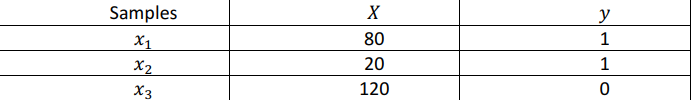
\includegraphics{1.png}
\caption{}
\end{figure}

\begin{itemize}
\item
  \begin{enumerate}
  \def\labelenumi{\alph{enumi})}
  \tightlist
  \item
    (10\%) Calculate the probability that \(y = 1\) for each \(x_i\) of
    the data set \((ℎ_{\theta }(x))\).
  \end{enumerate}
\item
  \begin{enumerate}
  \def\labelenumi{\alph{enumi})}
  \setcounter{enumi}{1}
  \tightlist
  \item
    (10\%) Calculate the value of objective (cost) function based on
    idea of SSE,
  \end{enumerate}
\item
  \begin{enumerate}
  \def\labelenumi{\alph{enumi})}
  \setcounter{enumi}{2}
  \tightlist
  \item
    (10\%) Calculate the value of objective (cost) function based on log
    of Sigmoid.
  \end{enumerate}
\end{itemize}

    For logistic regression learning:

\begin{enumerate}
\def\labelenumi{(\alph{enumi})}
\item
\end{enumerate}

\[h_\theta(x_1) = P(y=1|x_1, \theta) = \frac{1}{1+ e^{-\theta^T x}} = \frac{1}{e^{-\theta_0 - \theta_1 \cdot x_1}}\]

\[ = \frac{1}{e^{-14 + 0.14 \cdot 80}} = 0.943\]

\[h_\theta(x_2) = P(y=1|x_2, \theta) = \frac{1}{1+ e^{-\theta^T x}} = \frac{1}{e^{-\theta_0 - \theta_1 \cdot x_2}}\]

\[ = \frac{1}{e^{-14 + 0.14 \cdot 20}} = 1.000\]

\[h_\theta(x_3) = P(y=1|x, \theta) = \frac{1}{1+ e^{-\theta^T x}} = \frac{1}{e^{-\theta_0 - \theta_1 \cdot x_3}}\]

\[ = \frac{1}{e^{-14 + 0.14 \cdot 120}} = 0.057\]

    \begin{enumerate}
\def\labelenumi{(\alph{enumi})}
\setcounter{enumi}{1}
\item
\end{enumerate}

Object Function based on the idea of SSE:

\[J(\theta) = J(\theta_0, \theta_1, ..., \theta_n) = \frac{1}{2m} \sum^m_{i=1} (h_{\theta}(x^i) - y^i)^2, \text{ where } m = 3\]

Thus

\[J(\theta) = \frac{1}{2m} \sum^m_{i=1} (h_{\theta}(x^i) - y^i)^2 = \frac{1}{6} [ (0.943 - 1)^2 + (1.00 -1)^2 + (0.057 - 0)^2 ] = 0.001083\]

    \begin{enumerate}
\def\labelenumi{(\alph{enumi})}
\setcounter{enumi}{2}
\item
\end{enumerate}

Object Function based on the idea of log of sigmoid:

\begin{align}
Err(h_{\theta}(x), y) = 
\left\{\begin{matrix} - \log(h_{\theta}(x)), if \: y=1
\\ -\log(1-h_{\theta}(x)), if \: y=0
\end{matrix}\right.
\end{align}

So

\begin{equation}\label{eq:}
\begin{aligned}
J(h_{\theta}(x), y) &= \frac{1}{m} \sum^m_{i=1} Err(h_{\theta}(x), y) \\
&= - \frac{1}{m} \sum^m_{i=1}\left [ y ^i \log(h_{\theta}(x^i)) + (1-y^i) (\log(1-h_{\theta}(x^i)) \right ] \\
&= - \frac{1}{m} [1 \cdot \log(0.943) + 1 \cdot \log 1 + 1 \cdot \log(1-0.057)] \\
&= 0.0564
\end{aligned}
\end{equation}

    \subsubsection*{Q2}\label{q2}

    \textbf{Decision Tree}

\begin{enumerate}
\def\labelenumi{\arabic{enumi}.}
\setcounter{enumi}{1}
\tightlist
\item
  Consider the following data set for binary class problem.
\end{enumerate}

\begin{figure}[H]
\centering
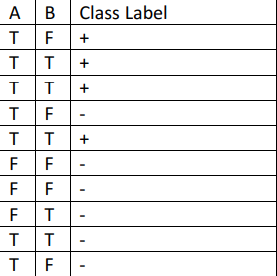
\includegraphics{2.png}
\caption{}
\end{figure}

\begin{itemize}
\item
  \begin{enumerate}
  \def\labelenumi{\alph{enumi}.}
  \tightlist
  \item
    (15\%) Calculate the information gain (based on entropy) when
    splitting on A and B. Which attribute would the decision tree
    induction algorithm choose?
  \end{enumerate}
\item
  \begin{enumerate}
  \def\labelenumi{\alph{enumi}.}
  \setcounter{enumi}{1}
  \tightlist
  \item
    (15\%) Calculate the gain (based on the Gini index) when splitting
    on A and B. Which attribute would the decision tree induction
    algorithm choose?
  \end{enumerate}
\end{itemize}

    \begin{enumerate}
\def\labelenumi{(\alph{enumi})}
\item
\end{enumerate}

\begin{table}[H]
\centering	
\begin{tabular}{|r|l|l|}

  & A=T & A=F \\
\hline
     C1=+ &  4     & 0 \\
     C2=-   &  3    & 3 \\
\end{tabular}
\end{table}


\begin{table}[H]
	\centering
\begin{tabular}{|r|l|l|}
  & B=T & B=F \\
\hline
     C1=+ &  3    & 1 \\
     C2=-   &  2    & 4 \\
\end{tabular}
\end{table}

\begin{itemize}
\tightlist
\item
  entropy before split:

  \begin{itemize}
  \tightlist
  \item[*]
    \[E = -0.4 \log (0.4) - 0.6 \log (0.6) = 0.971\]
  \item[*]
    entropy after splitting on A:

    \begin{itemize}
    \tightlist
    \item[*]
      \[E(A_T) = -\frac{4}{7} \log \frac{4}{7} - \frac{3}{7} \log \frac{3}{7} = 0.985\]
    \item
      \[E(A_F) = - \frac{3}{3} \log \frac{3}{3} = 0 \]
    \item
      info gain(A):
      \[E - \frac{7}{10} E(A_T) - \frac{3}{10} E(A_F) = 0.971 - 0.7 \cdot 0.985 = 0.2815\]
    \end{itemize}
  \item[*]
    entropy after splitting on B:

    \begin{itemize}
    \tightlist
    \item
      \[E(B_T) = -\frac{3}{5} \log \frac{3}{5} - \frac{2}{5} \log \frac{2}{5} = 0.971\]
    \item
      \[E(B_F) = - \frac{1}{5} \log \frac{1}{5} - \frac{4}{5} \log \frac{4}{5} = 0.722\]
    \item
      info gain(B):
      \[E - \frac{5}{10} E(B_T) - \frac{5}{10} E(B_F) = 0.971 - 0.5 \cdot 0.971 - 0.5 \cdot 0.722 = 0.1245\]
    \end{itemize}
  \end{itemize}
\end{itemize}

Since \(info \: gain(A) = 0.2815 > info \: gain(B) = 0.1245\), so if
split on A, the reduction of entropy, i.e. the reduction of uncertainty
is larger than if split on B. Thus \textbf{A should be selected for the
Decision Tree.}

    \begin{enumerate}
\def\labelenumi{(\alph{enumi})}
\setcounter{enumi}{1}
\item
\end{enumerate}

\begin{itemize}
\tightlist
\item
  Gini before split:

  \begin{itemize}
  \tightlist
  \item[*]
    \[G = 1- 0.4^2 - 0.6^2 = 0.48\]
  \item[*]
    Gini after splitting on A:

    \begin{itemize}
    \tightlist
    \item
      \[G(A_T) = 1-(\frac{4}{7})^2 - (\frac{3}{7}) ^2 = 0.4898\]
    \item
      \[G(A_F) = 1 - (\frac{3}{3})^2 - (\frac{0}{3})^2 = 0 \]
    \item
      info gain(A):
      \[G - \frac{7}{10} G(A_T) - \frac{3}{10} G(A_F) = 0.48 - 0.7 \cdot 0.4898= 0.137\]
    \end{itemize}
  \item[*]
    Gini after splitting on B:

    \begin{itemize}
    \tightlist
    \item
      \[G(B_T) = 1 -(\frac{3}{5})^2 - (\frac{2}{5})^2 = 0.48\]
    \item
      \[G(B_F) = 1- (\frac{1}{5})^2 - (\frac{4}{5})^2 = 0.32\]
    \item
      info gain(B):
      \[G - \frac{5}{10} G(B_T) - \frac{5}{10} G(B_F) = 0.48 - 0.5 \cdot 0.48 - 0.5 \cdot 0.32 = 0.08\]
    \end{itemize}
  \end{itemize}
\end{itemize}

Since \(info \: gain(A) = 0.137 > info \: gain(B) = 0.08\), so if split
on A, the reduction of Gini, i.e. the reduction of uncertainty is larger
than if split on B. Thus \textbf{A should be selected for the Decision
Tree.}

    \subsubsection*{Q3}\label{q3}

    The following table summarizes a data set with three attributes A, B, C
and two class labels +, − . Build a two-level decision tree.

\begin{figure}[H]
\centering
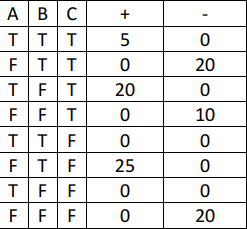
\includegraphics{3.png}
\caption{}
\end{figure}

\begin{itemize}
\item
  \begin{enumerate}
  \def\labelenumi{\alph{enumi}.}
  \tightlist
  \item
    (15\%) According to the classification error rate, which attribute
    would be chosen as the first splitting attribute? For each
    attribute, show the contingency table (i.e., count matrix) and the
    gains in classification error rate.
  \end{enumerate}
\item
  \begin{enumerate}
  \def\labelenumi{\alph{enumi}.}
  \setcounter{enumi}{1}
  \tightlist
  \item
    (15\%) Repeat for the two children of the root node.
  \end{enumerate}
\item
  \begin{enumerate}
  \def\labelenumi{\alph{enumi}.}
  \setcounter{enumi}{2}
  \tightlist
  \item
    (10\%) How many instances are misclassified by the resulting
    decision tree?
  \end{enumerate}
\end{itemize}

    \begin{enumerate}
\def\labelenumi{(\alph{enumi})}
\item
\end{enumerate}

\begin{table}[H]
	\centering
\begin{tabular}{|r|l|l|}
  & A=T & A=F \\
\hline
     C1=+ &  25     & 25 \\
     C2=-   &  0    & 50 \\
\end{tabular}
\end{table}

\begin{table}[H]
	\centering
\begin{tabular}{|r|l|l|}
  & B=T & B=F \\
\hline
     C1=+ &  30    & 20 \\
     C2=-   &  20    & 30 \\
\end{tabular}
\end{table}

\begin{table}[H]
	\centering
\begin{tabular}{|r|l|l|}
  & C=T & C=F \\
\hline
     C1=+ &  25    & 25 \\
     C2=-   &  30    & 20 \\
\end{tabular}
\end{table}

\begin{itemize}
\tightlist
\item
  Error before split:

  \begin{itemize}
  \tightlist
  \item[*]
    \[Err = 1-\max(\frac{50}{100}, \frac{50}{100}) = 0.5\]
  \item[*]
    Error after splitting on A:

    \begin{itemize}
    \tightlist
    \item
      \[Err(A_T) = 1-\max(\frac{25}{25}, \frac{0}{25}) = 0\]
    \item
      \[Err(A_F) = 1-\max(\frac{25}{75}, \frac{50}{75}) = 0.333\]
    \item
      \[\Delta Err(A) = Err- \frac{25}{100} \cdot Err(A_T) - \frac{75}{100} \cdot Err(A_F) = 0.5 - 0.75 \cdot 0.333 = 0.25025\]
    \end{itemize}
  \item[*]
    Error after splitting on B:

    \begin{itemize}
    \tightlist
    \item[*]
      \[Err(B_T) = 1-\max(\frac{30}{50}, \frac{20}{50}) = 0.4\]
    \item
      \[Err(B_F) = 1-\max(\frac{20}{50}, \frac{30}{50}) = 0.4\]
    \item
      \[\Delta Err(B) = Err- \frac{50}{100} \cdot Err(B_T) - \frac{50}{100} \cdot Err(B_F) = 0.5 - 0.5 \cdot 0.4 \cdot 2 = 0.1\]
    \end{itemize}
  \item[*]
    Error after splitting on C:

    \begin{itemize}
    \tightlist
    \item
      \[Err(C_T) = 1-\max(\frac{25}{55}, \frac{30}{55}) = 0.455\]
    \item
      \[Err(C_F) = 1-\max(\frac{25}{45}, \frac{20}{45}) = 0.444\]
    \item
      \[\Delta Err(C) = Err- \frac{55}{100} \cdot Err(C_T) - \frac{45}{100} \cdot Err(C_F) = 0.5 - 0.55 \cdot 0.455 - 0.45 \cdot 0.444 = 0.04995\]
    \end{itemize}
  \end{itemize}
\end{itemize}

Since \(\Delta Err(A) \textgreater{} \Delta Err(B) \textgreater{}
\Delta Err(C) \), thus attribute A should be chosen as the first
splitting attribute.

    \begin{enumerate}
\def\labelenumi{(\alph{enumi})}
\setcounter{enumi}{1}
\item
\end{enumerate}

\begin{itemize}
\tightlist
\item
  first child

  \begin{itemize}
  \tightlist
  \item[*]
    \(A=T\) is pure and no further split is required
  \item[*]
    \(A=F\)
  \end{itemize}
\end{itemize}


\begin{table}[H]
	\centering
\begin{tabular}{|r|l|l|}
              & B=T & B=F \\
            \hline
                 C1=+ &  25    & 0 \\
                 C2=-   &  20    & 30 \\
\end{tabular}
\end{table}

\begin{table}[H]
	\centering
\begin{tabular}{|r|l|l|}
              & C=T & C=F \\
            \hline
                 C1=+ &  0    & 25 \\
                 C2=-   &  30    & 20 \\
\end{tabular}
\end{table}

\begin{itemize}
\tightlist
\item
  Error before split:

  \begin{itemize}
  \tightlist
  \item[*]
    \[Err = 1-\max(\frac{25}{75}, \frac{50}{75}) = 0.333\]
  \end{itemize}
\item[*]
  Error after splitting on B:

  \begin{itemize}
  \tightlist
  \item[*]
    \[Err(B_T) = 1-\max(\frac{25}{45}, \frac{20}{45}) = 0.444\]
  \item[*]
    \[Err(B_F) = 1-\max(\frac{0}{30}, \frac{30}{30}) = 0\]
  \item[*]
    \[\Delta Err(B) = Err- \frac{45}{75} \cdot Err(B_T) - \frac{30}{75} \cdot Err(B_F) = 0.333 - 0.6  \cdot 0.444 - 0.4 \cdot 0 = 0.0666\]
  \end{itemize}
\item[*]
  Error after splitting on C:

  \begin{itemize}
  \tightlist
  \item[*]
    \[Err(C_T) = 1-\max(\frac{0}{30}, \frac{30}{30}) = 0\]
  \item[*]
    \[Err(C_F) = 1-\max(\frac{25}{45}, \frac{20}{45}) = 0.444\]
  \item[*]
    \[\Delta Err(C) = Err- \frac{30}{75} \cdot Err(C_T) - \frac{45}{75} \cdot Err(C_F) = 0.333 - 0.4 \cdot 0 - 0.6 \cdot 0.444 = 0.0666\]
  \end{itemize}
\end{itemize}



    \begin{enumerate}
\def\labelenumi{(\alph{enumi})}
\setcounter{enumi}{2}
\item
\end{enumerate}

from part B:

\begin{itemize}
\tightlist
\item
  if B is the second child
\end{itemize}

\begin{figure}[H]
	\centering
	
\includegraphics{7.png}
	\caption{}
\end{figure}

\textbf{misclassified instances = 20}

\begin{itemize}
\tightlist
\item
  if C is the second child
\end{itemize}

\begin{figure}[H]
\centering
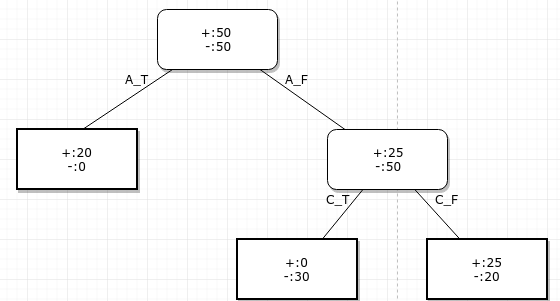
\includegraphics{6.png}
\caption{}
\end{figure}

\textbf{misclassified instances = 20}
\\\\
So, in conclusion, there are 20 misclassified instances from this decision
tree.


But if the splitting continues, 

\begin{figure}[H]
	\centering
	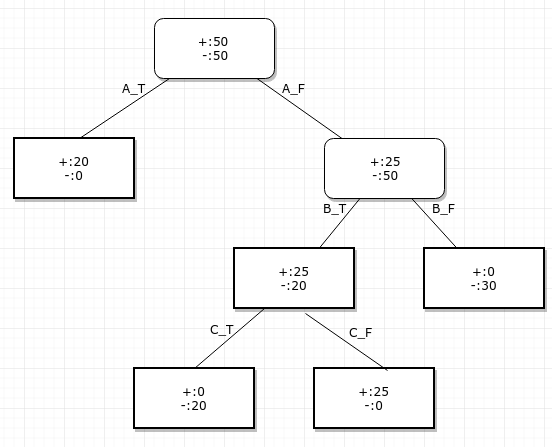
\includegraphics{4.png}
	\caption{}
\end{figure}

\begin{figure}[H]
	\centering
	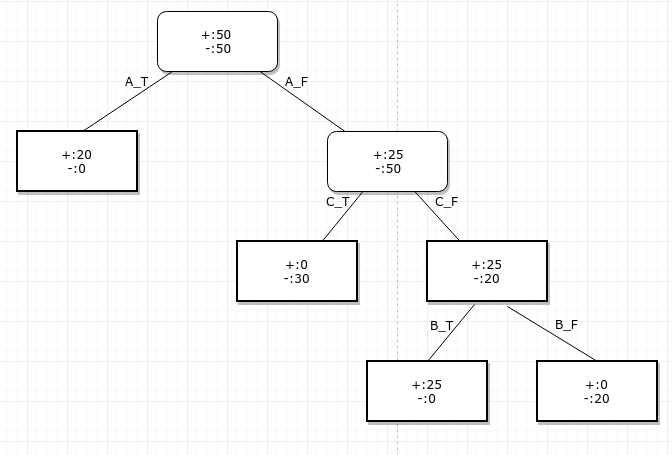
\includegraphics{5.png}
	\caption{}
\end{figure}

Then we might be able to reduce the misclassified instance to 0.

    % Add a bibliography block to the postdoc
    
    
    
    \end{document}
